
%it will be clear from the preceding examples that is is by no means easy to determine whether G is a subgraph of G*-v.
\section{requesting survival virtual network using integer linear programming}
\label{sec:SVN_ILP}
The one of contributions of this paper is the modelization of specific node fault tolerant problem as an optimization. The general technique used to solve this problem is a combined algorithm consisting of enumeration and Ullmann Algorithm\cite{ullmann1976algorithm}, which is proposed as a  algorithm of exponential complexity which is brute force method briefly. More precisely, we propose an Integer Linear Program(ILP)\cite{schrijver1998theory} model of this problem. In the following, We briefly explain how to solve a problem using ILP.

\subsection{Modeling the SNFT problem}
In this section, we formulate the problems discussed in the previous sections with Integer Linear Program(ILP) method. Though we have proved that these problems are NP-complete, as we will demonstrate later, the ILP formulation of the problem provides a very viable tool for solving it, for most real-world virtual network request which typically have less than a few hundred nodes and edges. Throughout this section, we will focus exclusively on the survival virtual network request [$G(V,E,S),B(V,S))$], we assume that $G$ is simple directed service label graph.
%the term graph represents a loop undirected non multidigraph. As a consequence, an edge e originating from i and targeting to j and can be denoted ij without any ambiguity.

%In order to model the problem as an ILP, we use binary variables, i.e. C=$\{0,1\}^n$
%transform the graph for reduce the constrain condition of service function.\ref{fig:ILP_transfromed_graph},\ref{fig:ILP_inserted_augmented_transformed_graph}.

To begin with, we introduce some necessary notation:

$MBG$: $[mbg_{u,v}]_{(|V|+|B|)\times (|V|+|B|)}$, the adjacency matrix of graph $G^o$. where

${mbg_{u,v}}=\left\{ \begin{array}{l}
1\ if\ edge\ e\ originates\ from\ u\ to\ v\\
0\ otherwise
\end{array} \right.$ \\

$MAG$: $[mag_{u,v}]_{|V|\times |V|}$, the adjacency matrix of arbitrary graph $G$. Where

${mag_{u,v}}=\left\{ \begin{array}{l}
1\ if\ edge\ e\ originates\ from\ u\ to\ v\\
0\ otherwise
\end{array} \right.$ \\

%matrix of service functions set corresponding to node
$T^{l}$: $[t^l_{u,v}]_{|V|\times (|V|+|B|)}$, The $l$-th node permutation matrix against $l$-th node failed. Where

${t^l_{u,v}}=\left\{ \begin{array}{l}1\ if\ node\ u\ transformed\ to\ node\ v\\
0\ otherwise
\end{array} \right.$.

$MBS$: $[mbs_{u,v}]_{(|V|+|B|)\times |S|}$, incidence matrix of specific services of the SNFT graph $G^o$. where

${mbs_{u,v}}=\left\{ \begin{array}{l}1\ if\ node\ u\ have\ specific\ flag\ v\\
0\ otherwise
\end{array} \right.$.

$MAS$: $[mas_{u,v}]_{|V|\times |S|}$, incidence matrix of  specific services of the arbitrary graph $G$. where

${mas_{u,v}}=\left\{ \begin{array}{l}1\ if\ node\ u\ have\ specific\ flag\ v\\
0\ otherwise
\end{array} \right.$.

$AugB$:$[aug_i]_{|B|}$, whether the i-th backup nodes is used or not. where

${aug_i}=\left\{ \begin{array}{l}1\ if\ node\ i\ is\ used\\
0\ otherwise
\end{array} \right.$.

The problem of requesting 1-specific node fault tolerant graph [$G(V,E,S),B(V,S))$] can be formulated as the folowing ILP problem:
\begin{center}
\begin{align}
\label{equ:ILPC1}such\ as:\ T^l*(T^l* MBG)^{'}&\geq MAG\\
\label{equ:ILPC2} \sum_{1\leq v\leq (n+b)}T^l_{iv}&= 1 (1\leq i\leq n)\\
\sum_{1\leq u\leq n}T^l_{uj}&\leq 1 (1\leq j\leq (n+b)) \notag \\
\sum_{1\leq u\leq n,1\leq v\leq (n+b)}T^l_{uv}&=n \notag\\
\label{equ:ILPC5}  T^k_{uk}&=0 (1\leq u\leq n)\\
\label{equ:ILPC7} MAG_{uv}&\leq MBG_{uv}(1\leq u\leq n,1\leq v\leq n)\\
\label{equ:ILPC8} MAS&\leq T^l*MBS\\
\label{equ:ILPC9} \frac{\sum_{1\leq v\leq (n+b)}MBG_{(n+i)v}+n-1}{n} &\leq B_i(1\leq i\leq b)\\
\end{align}

\end{center}

\begin{itemize}
\item Constraint(\ref{equ:ILPC1}) guarantees that when the l-th critical node of graph $G$ failed, we could find subgraph which is subgraph isomorphism of SNFT graph $G^o$. we represent the mapping relation as permutation matrix in view of Ullman\cite{ullmann1976algorithm}
\item Constraint(\ref{equ:ILPC5}) implies that operation of the transform matrix of mapping relation is appropriate and correct format in respect with one node failure.
\item Constraint(\ref{equ:ILPC7}) guarantees that SNFT graph $G^o$ must be the augmented graph of previous graph $G$.
\item Constraint(\ref{equ:ILPC8}) guarantees that when the l-th node failed  all nodes of the transformed graph still have specific flag, which is specific flag of corresponding node of previous graph $G$.

\end{itemize}
%
%\begin{figure}
%\centering
%% Requires \usepackage{graphicx}
%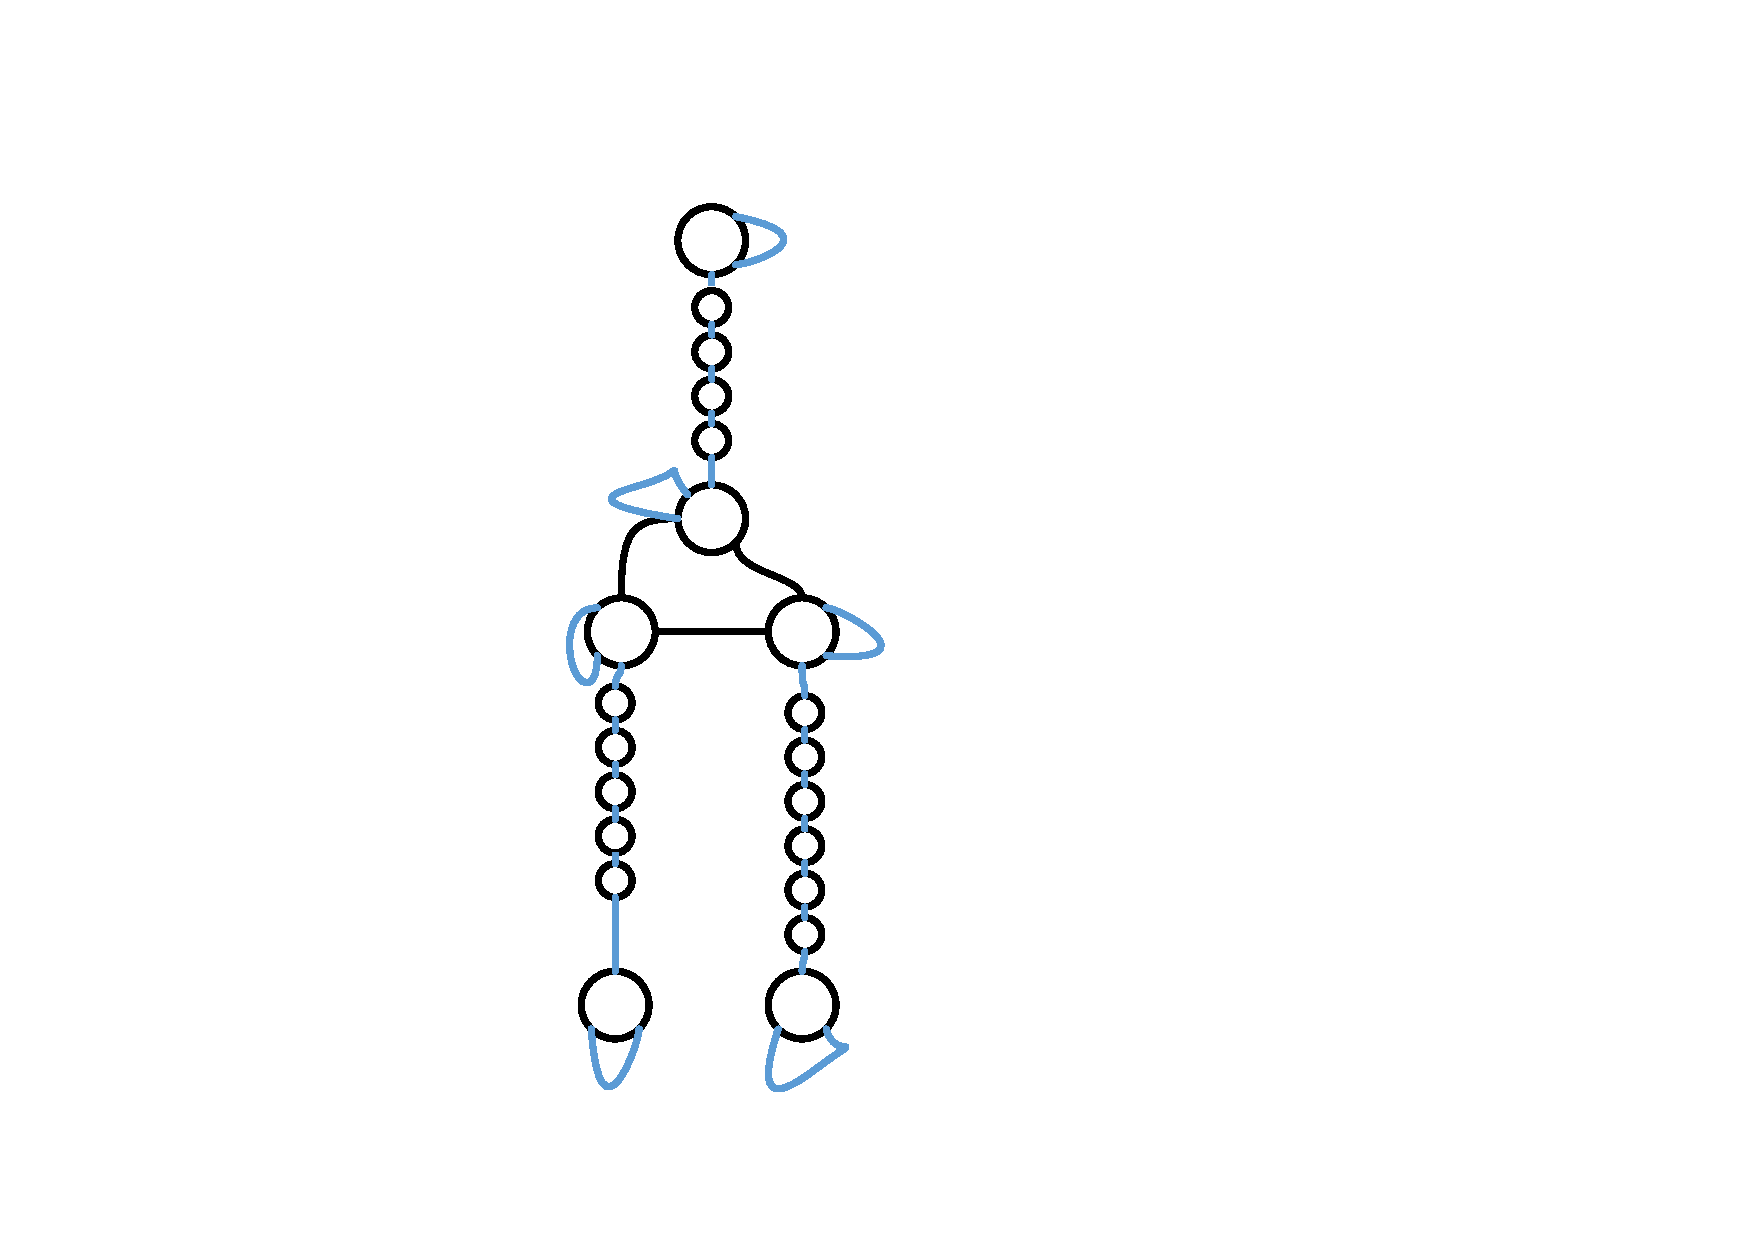
\includegraphics[width=2.5in]{ILP_transfromed_graph}\\
%\caption{transformed Graph G}\label{fig:ILP_transfromed_graph}
%\end{figure}
%
%\begin{figure}
%\centering
%% Requires \usepackage{graphicx}
%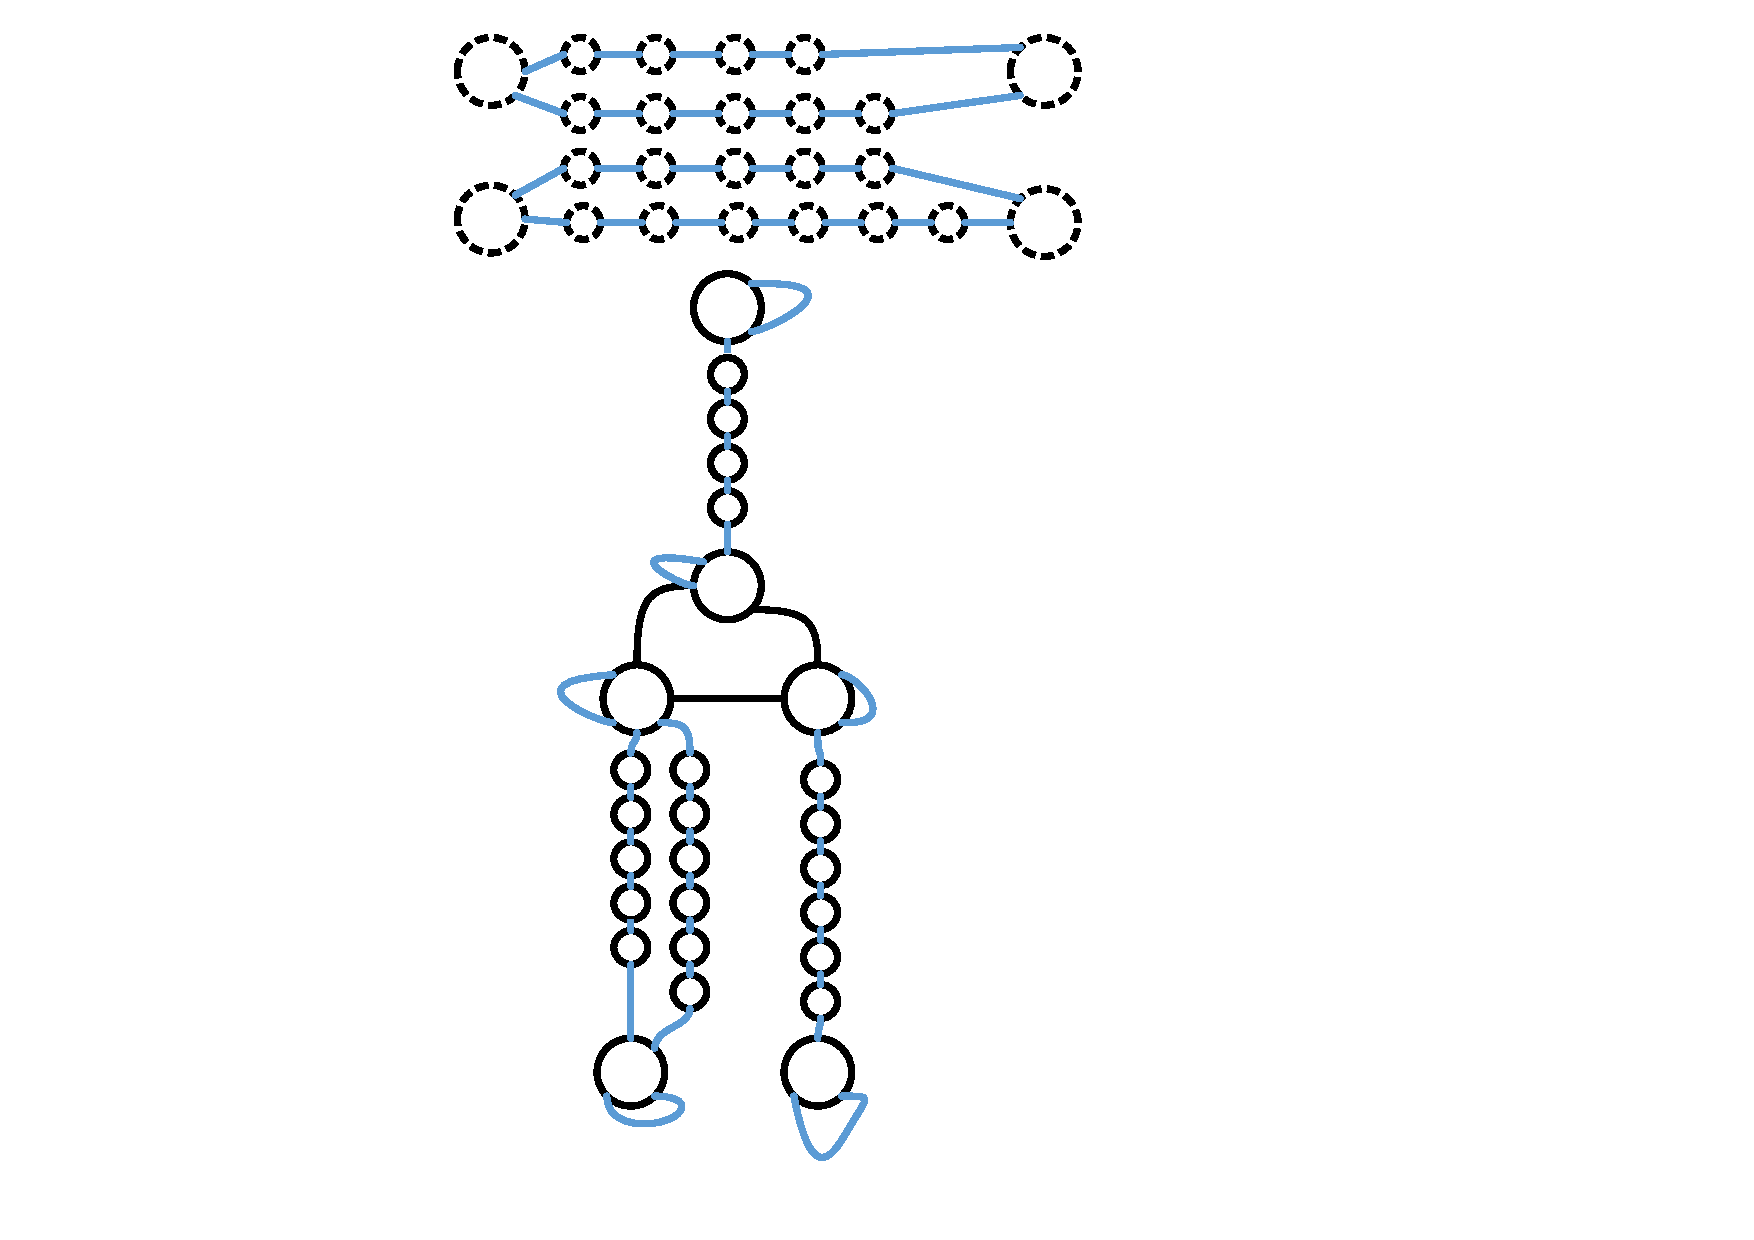
\includegraphics[width=2.5in]{ILP_inserted_augmented_transformed_graph}\\
%\caption{transformed Graph of to be augmented graph G}\label{fig:ILP_inserted_augmented_transformed_graph}
%\end{figure}

\subsection{Objective Function and Approximation}
We seek to minimize the amount of resource used for a VInf. The object function of the adapted ILP is then
\begin{align}
min: \alpha \sum_{1\leq i\leq b}B_i+ & \notag \\
\beta \times(\sum_{1\leq u\leq (n+b) 1\leq v\leq (n+b)}MBG_{uv}-&\sum_{1\leq u\leq n,1\leq v\leq n}MAG_{uv})
\end{align}
where $\alpha$ and $\beta$ are node and link weights, respectively. To achieve minimize the amount of nodes, the weight can be set as $(n^2+1)$ and $1$, respectively.

The presence of the boolean variables turns the linear program into a NP-Hard problem. An alterative is to relax the boolean variables to real-value variables, obtain an approximate virtual node transformation.




\begin{equation}
dp[i][{W_1}][{W_2}] \ldots [{W_m}] = \left\{ \begin{array}{l}
dp[i - 1][{W_1} - {w_i}][{W_2}] \ldots [{W_m}] + {v_i}\\
dp[i - 1][W][{W_2}_{} - {w_i}] \ldots [{W_m}] + {v_i}\\
dp[i - 1][W][{W_2}_{}] \ldots [{W_m} - {w_i}] + {v_i}
\end{array} \right\}
\end{equation}

$n*\prod_{i=1}^mC_i$

$m*n*\prod_{i=1}^mC_i$
